\chapter{Evaluation}

In this chapter, we will evaluate the strategies through performance
measurements and compare them with one another.

\section{Performance evaluation}

Performance measurements were taken for each strategy as well as for naive
reference implementations and are presented through latency $lat$ in cycles per
byte (c/B) as well as constant throughput $thr$ in MiB/s of the entire
encryption strategy. Round key derivation is measured separately. Measurements
of all individual components like packing or permuting have to be viewed as
upper bounds due to the aforementioned inlining, instruction reordering and
pipelining taking place in the actual encryption function.

ARMv8-A defines system registers in addition to general-purpose registers which
are used for system configuration and monitoring. One of these registers is the
performance monitor cycle count register \texttt{PMCCNTR} which counts
processor clock cycles. Access from userspace is disabled by default and can be
activated through a custom Linux kernel module by setting \texttt{PMUSERENR.EN}
to 1. To minimize interference and because the cycle count register is
core-local, we isolate and utilize one Cortex-A53 and Cortex-A73 core from the
rest of the system for exclusive benchmarking purposes respectively by use of
the \texttt{isolcpus} kernel command line parameter and \texttt{taskset}
command utility. Results can be found in full in Appendix \ref{app:benchmarks}
and are summarized in Figure \ref{figure:benchmark}.

\begin{figure}[h!]
    \centering
    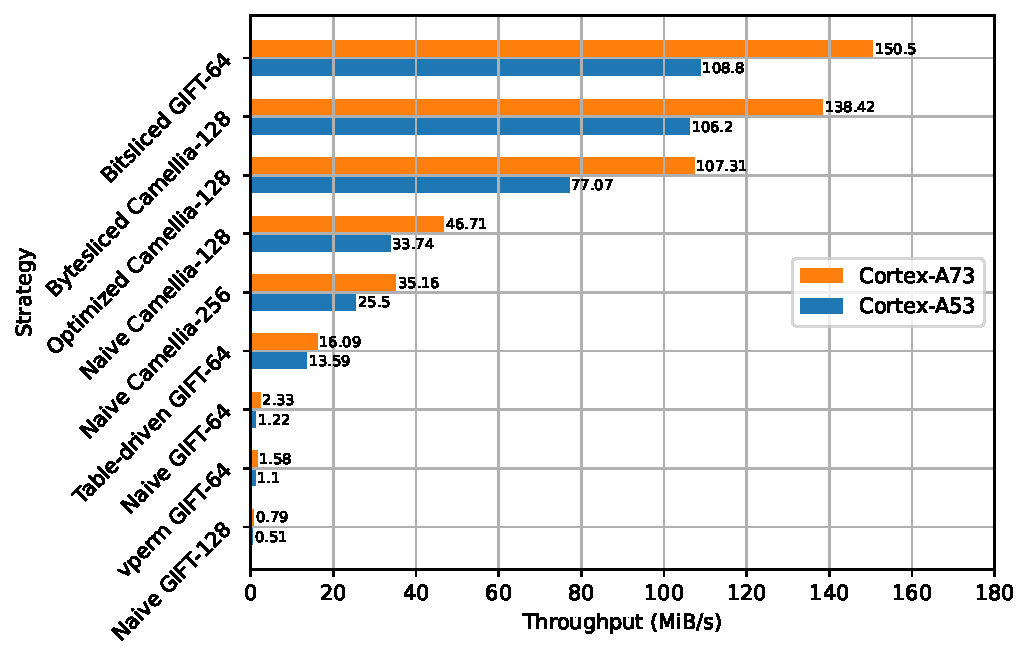
\includegraphics[width=\textwidth]{Figures/benchmark_plot.pdf}
    \caption{Throughput in MiB/s for each strategy and processor type}
    \label{figure:benchmark}
\end{figure}

Bit- and bytesliced implementations leveraging SIMD instructions show the
highest throughput values. Camellia implementations tend to be faster than GIFT
due to the higher number of rounds as well as the bit permutation slowing down
GIFT software implementations, differing from Camellia which is byte-oriented.
Bitsliced GIFT manages to be the fastest due to the bit permutation being
implemented efficiently through bytewise table lookups. Bytesliced Camellia
achieves an only slightly lower performance than bitsliced GIFT in spite of
increased complexity due to the higher number of bytes being encrypted in
parallel.

The claimed performance of GIFT by the original authors of 2.10 cycles per byte
utilizing Intel AVX2 is superior to our implementation which only manages to
achieve 13.98 cycles per byte \cite{gift:2017}.

Our Camellia implementation for ARMv8 achieves a latency of around 15.19 cycles
per byte, putting it in a similar position as the byte-sliced implementation
for x86 utilizing AVX and AES-NI instructions which claims a latency of 5.32
cycles per byte \cite{bcfastimplx86:2013} and surpassing the figure of 20.38
cycles per byte of the original Camellia paper \cite{camellia:2001}.

The differences in speed are grounded in varying vector register sizes,
instruction timings and implementation details as well as available vector
instructions.

Table-driven implementations show a $691\%$ and $230\%$ improvement for GIFT
and Camellia respectively compared to their naive implementations. GIFT
especially benefits from this approach due to the elimination of the expensive
bit permutation layer. While S-box lookup is accelerated for \texttt{vperm}
GIFT-64, the whole implementation only achieves a throughput of
$1.58\text{MiB/s}$ due to extremely inefficient packing and unpacking
operations every round.

\section{Conclusion}

We have examined various strategies for efficient implementation of GIFT and
Camellia and have realized these in the C programming language using NEON
intrinsics for the ARMv8 platform. Bit- and bytesliced implementations have
proven themselves especially suited for high-throughput applications on SIMD
platforms with the added security benefit of being constant-time, thus
eliminating possible side-channels through e.g. cache timings. Table
implementations also show good performance characteristics compared to
non-table approaches and are extremely easy to port to other platforms since
they don't rely on any specific machine instructions, but are vulnerable to
cache timing attacks since they access data-dependent memory locations.

GIFT as well as Camellia are suited for low-power hardware as well as bitsliced
software implementation with GIFT appearing to be more suited towards hardware
implementation due to the low area requirement of the S-box and bit wiring
permutation layer.

Vector length determines the number of blocks that can be processed in parallel
and therefore is the major contributor to performance since a doubling of
register size with the same instruction throughput generally implies a doubling
in performance. NEON provides 128 bit registers which is smaller than the 512
bit registers offered by Intel's AVX-512, but new extensions for ARM like SVE2
offer flexible vector lengths up to 2048 bits which will result not only in
further acceleration of traditional compute domains like machine learning or
multimedia, but also of massively parallelized cryptographic algorithms for
low-power and embedded systems.

\pagebreak

\section{Notes}

Working on this project has allowed me to learn a lot about ARMv8 and its A64
instruction set as well as SIMD extensions and the use of intrinsics. I have
written a lot of code for x86-64, but working with a RISC machine with
comparatively simple instructions and addressing modes felt somewhat simpler
and more straightforward. The toolchain was surprisingly simple to set up:
after flashing a custom odroid Linux image to the SD card, setting up SSH,
copying the sysroot (i.e. \texttt{/lib} and \texttt{/usr}) to my local
development machine and feeding clang with the correct parameters for
compilation, I could just copy the binary to the target system and run it
there. Building, deploying and executing was simple to automate using a
Makefile.

Aside from tooling, I also learned a lot about efficient cryptography
implementations and how bitslicing can make a seemingly inefficient cipher like
GIFT very fast. Most of the time debugging was spent on fixing values for
permutation tables since it was easy to make a mistake there, but once they
were corrected the rest was usually pretty simple.

Trying to optimize performance without writing assembler code was also very
educational since constantly making small adjustments to the C program and then
analyzing the disassembled binaries taught me a lot about what the compiler
actually does and how it optimizes programs through e.g. loop unrolling and
inlining as well as combining logical instructions.
